Representative samples from each ground-truth class in the dataset used to train the VAE. 
While the VAE is trained in an unsupervised manner (without class labels), the labels are shown here for reference to illustrate the visual diversity within and across the STOP, GO, LEFT, and RIGHT categories. This includes variations in viewpoint, lighting, and road layout. To illustrate the diversity present in the collected dataset, Figures~\ref{fig:diversity_stop_go} and~\ref{fig:diversity_left_right} show representative samples grouped by class labels available from CARLA. Although the VAE is trained unsupervised, this diversity impacts the quality of latent space representations.


\begin{figure}[htbp]
    
    \begin{tabular}{cccccccccc}
        \multicolumn{10}{c}{\textbf{STOP}} \\
        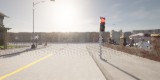
\includegraphics[width=0.2\textwidth]{img/diversity/stop_01.png} &
        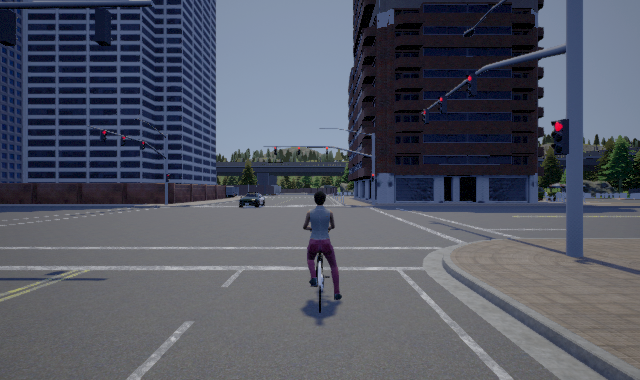
\includegraphics[width=0.2\textwidth]{img/diversity/stop_04.png} &
        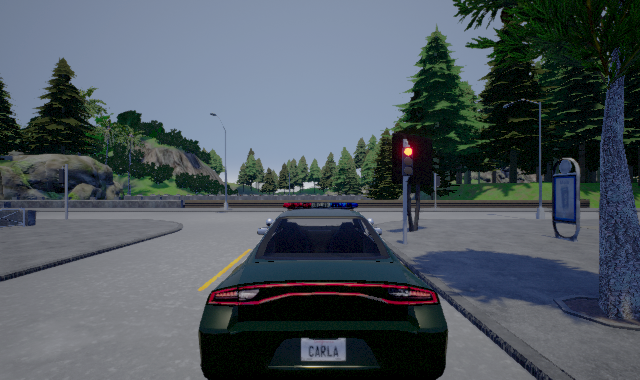
\includegraphics[width=0.2\textwidth]{img/diversity/stop_03.png} &
        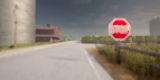
\includegraphics[width=0.2\textwidth]{img/diversity/stop_02.png} &
        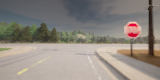
\includegraphics[width=0.2\textwidth]{img/diversity/stop_06.png} & \\
         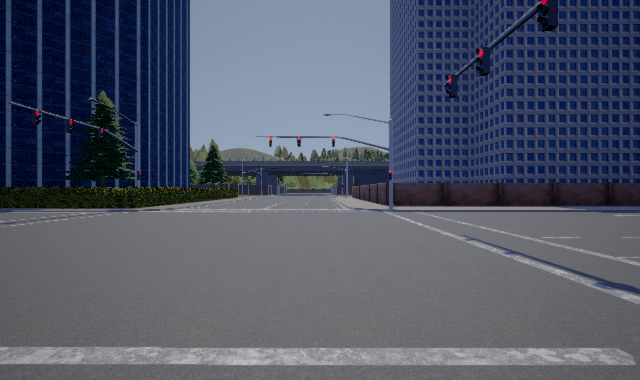
\includegraphics[width=0.2\textwidth]{img/diversity/stop_05.png} &
        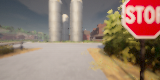
\includegraphics[width=0.2\textwidth]{img/diversity/stop_07.png} &
        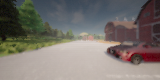
\includegraphics[width=0.2\textwidth]{img/diversity/stop_08.png} &
        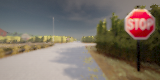
\includegraphics[width=0.2\textwidth]{img/diversity/stop_09.png} &
        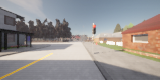
\includegraphics[width=0.2\textwidth]{img/diversity/stop_10.png} \\
        \multicolumn{10}{c}{\textbf{GO}} \\
        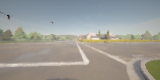
\includegraphics[width=0.2\textwidth]{img/diversity/go_01.png} &
        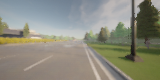
\includegraphics[width=0.2\textwidth]{img/diversity/go_02.png} &
        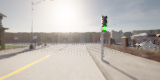
\includegraphics[width=0.2\textwidth]{img/diversity/go_03.png} &
        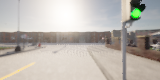
\includegraphics[width=0.2\textwidth]{img/diversity/go_04.png} &
        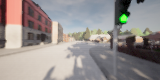
\includegraphics[width=0.2\textwidth]{img/diversity/go_05.png} & \\
        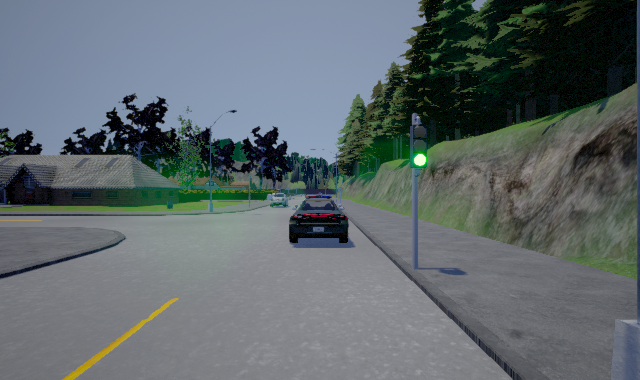
\includegraphics[width=0.2\textwidth]{img/diversity/go_06.png} &
        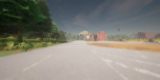
\includegraphics[width=0.2\textwidth]{img/diversity/go_07.png} &
        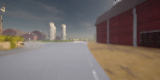
\includegraphics[width=0.2\textwidth]{img/diversity/go_08.png} &
        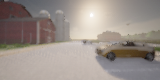
\includegraphics[width=0.2\textwidth]{img/diversity/go_09.png} &
        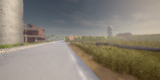
\includegraphics[width=0.2\textwidth]{img/diversity/go_10.png} \\
    \end{tabular}
    \caption[Dataset diversity — STOP and GO classes]{%
Representative samples from the \texttt{STOP} and \texttt{GO} classes in the dataset. Although the VAE was trained in an unsupervised manner, these class-labeled examples illustrate the visual diversity captured during training.}
    \label{fig:diversity_stop_go}
\end{figure}


\begin{figure}[htbp]
    \begin{tabular}{cccccccccc}
        \multicolumn{10}{c}{\textbf{LEFT}} \\
        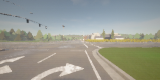
\includegraphics[width=0.2\textwidth]{img/diversity/left_01.png} &
        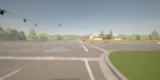
\includegraphics[width=0.2\textwidth]{img/diversity/left_02.png} &
        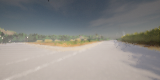
\includegraphics[width=0.2\textwidth]{img/diversity/left_07.png} &
        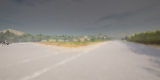
\includegraphics[width=0.2\textwidth]{img/diversity/left_04.png} &
        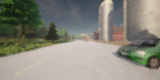
\includegraphics[width=0.2\textwidth]{img/diversity/left_09.png} & \\
        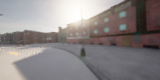
\includegraphics[width=0.2\textwidth]{img/diversity/left_06.png} &
        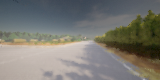
\includegraphics[width=0.2\textwidth]{img/diversity/left_03.png} &
        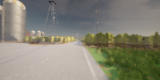
\includegraphics[width=0.2\textwidth]{img/diversity/left_08.png} &
        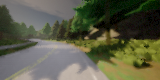
\includegraphics[width=0.2\textwidth]{img/diversity/left_05.png} &
        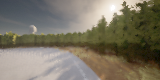
\includegraphics[width=0.2\textwidth]{img/diversity/left_10.png} \\
        
        \multicolumn{10}{c}{\textbf{RIGHT}} \\
        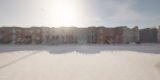
\includegraphics[width=0.2\textwidth]{img/diversity/right_01.png} &
        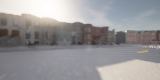
\includegraphics[width=0.2\textwidth]{img/diversity/right_02.png} &
        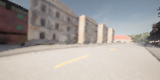
\includegraphics[width=0.2\textwidth]{img/diversity/right_03.png} &
        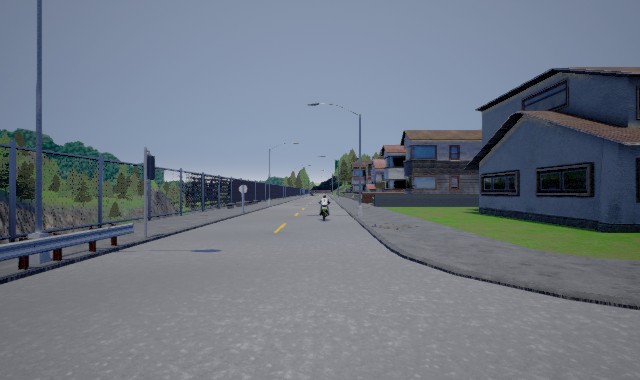
\includegraphics[width=0.2\textwidth]{img/diversity/right_04.png} &
        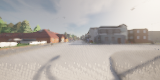
\includegraphics[width=0.2\textwidth]{img/diversity/right_05.png} & \\
        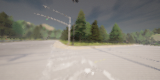
\includegraphics[width=0.2\textwidth]{img/diversity/right_06.png} &
        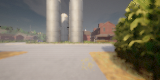
\includegraphics[width=0.2\textwidth]{img/diversity/right_07.png} &
        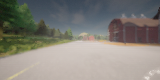
\includegraphics[width=0.2\textwidth]{img/diversity/right_08.png} &
        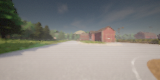
\includegraphics[width=0.2\textwidth]{img/diversity/right_09.png} &
        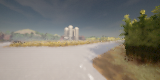
\includegraphics[width=0.2\textwidth]{img/diversity/right_10.png} \\
    \end{tabular}
    \caption[Dataset diversity — LEFT and RIGHT classes]{%
Representative samples from the \texttt{LEFT} and \texttt{RIGHT} classes. These examples highlight road turns under varying lighting and scene layouts.}
    \label{fig:diversity_left_right}
\end{figure}
